%% bare_jrnl.tex
%% V1.4b
%% 2015/08/26
%% by Michael Shell
%% see http://www.michaelshell.org/
%% for current contact information.
%%
%% This is a skeleton file demonstrating the use of IEEEtran.cls
%% (requires IEEEtran.cls version 1.8b or later) with an IEEE
%% journal paper.
%%
%% Support sites:
%% http://www.michaelshell.org/tex/ieeetran/
%% http://www.ctan.org/pkg/ieeetran
%% and
%% http://www.ieee.org/

%%*************************************************************************
%% Legal Notice:1
%% This code is offered as-is without any warranty either expressed or
%% implied; without even the implied warranty of MERCHANTABILITY or
%% FITNESS FOR A PARTICULAR PURPOSE! 
%% User assumes all risk.
%% In no event shall the IEEE or any contributor to this code be liable for
%% any damages or losses, including, but not limited to, incidental,
%% consequential, or any other damages, resulting from the use or misuse
%% of any information contained here.
%%
%% All comments are the opinions of their respective authors and are not
%% necessarily endorsed by the IEEE.
%%
%% This work is distributed under the LaTeX Project Public License (LPPL)
%% ( http://www.latex-project.org/ ) version 1.3, and may be freely used,
%% distributed and modified. A copy of the LPPL, version 1.3, is included
%% in the base LaTeX documentation of all distributions of LaTeX released
%% 2003/12/01 or later.
%% Retain all contribution notices and credits.
%% ** Modified files should be clearly indicated as such, including  **
%% ** renaming them and changing author support contact information. **
%%*************************************************************************


% *** Authors should verify (and, if needed, correct) their LaTeX system  ***
% *** with the testflow diagnostic prior to trusting their LaTeX platform ***
% *** with production work. The IEEE's font choices and paper sizes can   ***
% *** trigger bugs that do not appear when using other class files.       ***                          ***
% The testflow support page is at:
% http://www.michaelshell.org/tex/testflow/


% Please refer to your journal's instructions for other
% options that should be set.
\documentclass[journal,twocolumn]{IEEEtran}
%
% If IEEEtran.cls has not been installed into the LaTeX system files,
% manually specify the path to it like:
% \documentclass[journal]{../sty/IEEEtran}





% Some very useful LaTeX packages include:
% (uncomment the ones you want to load)


% *** MISC UTILITY PACKAGES ***
%
%\usepackage{ifpdf}
% Heiko Oberdiek's ifpdf.sty is very useful if you need conditional
% compilation based on whether the output is pdf or dvi.
% usage:
% \ifpdf
%   % pdf code
% \else
%   % dvi code
% \fi
% The latest version of ifpdf.sty can be obtained from:
% http://www.ctan.org/pkg/ifpdf
% Also, note that IEEEtran.cls V1.7 and later provides a builtin
% \ifCLASSINFOpdf conditional that works the same way.
% When switching from latex to pdflatex and vice-versa, the compiler may
% have to be run twice to clear warning/error messages.


\usepackage{pgfplots}
\usepackage{pgfplotstable}
\pgfplotsset{compat=1.17}

\usepackage{booktabs}

\usepackage{comment}

\usepackage{xcolor}

\definecolor{redbullet}{RGB}{234,67,53}
\definecolor{bluebullet}{RGB}{66,133,244}
\definecolor{yellowbullet}{RGB}{251,188,4}
\definecolor{greenbullet}{RGB}{52,168,83}

% *** CITATION PACKAGES ***
%
%\usepackage{cite}
% cite.sty was written by Donald Arseneau
% V1.6 and later of IEEEtran pre-defines the format of the cite.sty package
% \cite{} output to follow that of the IEEE. Loading the cite package will
% result in citation numbers being automatically sorted and properly
% "compressed/ranged". e.g., [1], [9], [2], [7], [5], [6] without using
% cite.sty will become [1], [2], [5]--[7], [9] using cite.sty. cite.sty's
% \cite will automatically add leading space, if needed. Use cite.sty's
% noadjust option (cite.sty V3.8 and later) if you want to turn this off
% such as if a citation ever needs to be enclosed in parenthesis.
% cite.sty is already installed on most LaTeX systems. Be sure and use
% version 5.0 (2009-03-20) and later if using hyperref.sty.
% The latest version can be obtained at:
% http://www.ctan.org/pkg/cite
% The documentation is contained in the cite.sty file itself.






% *** GRAPHICS RELATED PACKAGES ***
%
\ifCLASSINFOpdf
  % \usepackage[pdftex]{graphicx}
  % declare the path(s) where your graphic files are
  % \graphicspath{{../pdf/}{../jpeg/}}
  % and their extensions so you won't have to specify these with
  % every instance of \includegraphics
  % \DeclareGraphicsExtensions{.pdf,.jpeg,.png}
\else
  % or other class option (dvipsone, dvipdf, if not using dvips). graphicx
  % will default to the driver specified in the system graphics.cfg if no
  % driver is specified.
  % \usepackage[dvips]{graphicx}
  % declare the path(s) where your graphic files are
  % \graphicspath{{../eps/}}
  % and their extensions so you won't have to specify these with
  % every instance of \includegraphics
  % \DeclareGraphicsExtensions{.eps}
\fi
% graphicx was written by David Carlisle and Sebastian Rahtz. It is
% required if you want graphics, photos, etc. graphicx.sty is already
% installed on most LaTeX systems. The latest version and documentation
% can be obtained at: 
% http://www.ctan.org/pkg/graphicx
% Another good source of documentation is "Using Imported Graphics in
% LaTeX2e" by Keith Reckdahl which can be found at:
% http://www.ctan.org/pkg/epslatex
%
% latex, and pdflatex in dvi mode, support graphics in encapsulated
% postscript (.eps) format. pdflatex in pdf mode supports graphics
% in .pdf, .jpeg, .png and .mps (metapost) formats. Users should ensure
% that all non-photo figures use a vector format (.eps, .pdf, .mps) and
% not a bitmapped formats (.jpeg, .png). The IEEE frowns on bitmapped formats
% which can result in "jaggedy"/blurry rendering of lines and letters as
% well as large increases in file sizes.
%
% You can find documentation about the pdfTeX application at:
% http://www.tug.org/applications/pdftex





% *** MATH PACKAGES ***
%
\usepackage{amsmath}
% A popular package from the American Mathematical Society that provides
% many useful and powerful commands for dealing with mathematics.
%
% Note that the amsmath package sets \interdisplaylinepenalty to 10000
% thus preventing page breaks from occurring within multiline equations. Use:
%\interdisplaylinepenalty=2500
% after loading amsmath to restore such page breaks as IEEEtran.cls normally
% does. amsmath.sty is already installed on most LaTeX systems. The latest
% version and documentation can be obtained at:
% http://www.ctan.org/pkg/amsmath





% *** SPECIALIZED LIST PACKAGES ***
%
\usepackage{algorithmic}
% algorithmic.sty was written by Peter Williams and Rogerio Brito.
% This package provides an algorithmic environment fo describing algorithms.
% You can use the algorithmic environment in-text or within a figure
% environment to provide for a floating algorithm. Do NOT use the algorithm
% floating environment provided by algorithm.sty (by the same authors) or
% algorithm2e.sty (by Christophe Fiorio) as the IEEE does not use dedicated
% algorithm float types and packages that provide these will not provide
% correct IEEE style captions. The latest version and documentation of
% algorithmic.sty can be obtained at:
% http://www.ctan.org/pkg/algorithms
% Also of interest may be the (relatively newer and more customizable)
% algorithmicx.sty package by Szasz Janos:
% http://www.ctan.org/pkg/algorithmicx




% *** ALIGNMENT PACKAGES ***
%
%\usepackage{array}
% Frank Mittelbach's and David Carlisle's array.sty patches and improves
% the standard LaTeX2e array and tabular environments to provide better
% appearance and additional user controls. As the default LaTeX2e table
% generation code is lacking to the point of almost being broken with
% respect to the quality of the end results, all users are strongly
% advised to use an enhanced (at the very least that provided by array.sty)
% set of table tools. array.sty is already installed on most systems. The
% latest version and documentation can be obtained at:
% http://www.ctan.org/pkg/array


% IEEEtran contains the IEEEeqnarray family of commands that can be used to
% generate multiline equations as well as matrices, tables, etc., of high
% quality.




% *** SUBFIGURE PACKAGES ***
%\ifCLASSOPTIONcompsoc
%  \usepackage[caption=false,font=normalsize,labelfont=sf,textfont=sf]{subfig}
%\else
%  \usepackage[caption=false,font=footnotesize]{subfig}
%\fi
% subfig.sty, written by Steven Douglas Cochran, is the modern replacement
% for subfigure.sty, the latter of which is no longer maintained and is
% incompatible with some LaTeX packages including fixltx2e. However,
% subfig.sty requires and automatically loads Axel Sommerfeldt's caption.sty
% which will override IEEEtran.cls' handling of captions and this will result
% in non-IEEE style figure/table captions. To prevent this problem, be sure
% and invoke subfig.sty's "caption=false" package option (available since
% subfig.sty version 1.3, 2005/06/28) as this is will preserve IEEEtran.cls
% handling of captions.
% Note that the Computer Society format requires a larger sans serif font
% than the serif footnote size font used in traditional IEEE formatting
% and thus the need to invoke different subfig.sty package options depending
% on whether compsoc mode has been enabled.
%
% The latest version and documentation of subfig.sty can be obtained at:
% http://www.ctan.org/pkg/subfig




% *** FLOAT PACKAGES ***
%
%\usepackage{fixltx2e}
% fixltx2e, the successor to the earlier fix2col.sty, was written by
% Frank Mittelbach and David Carlisle. This package corrects a few problems
% in the LaTeX2e kernel, the most notable of which is that in current
% LaTeX2e releases, the ordering of single and double column floats is not
% guaranteed to be preserved. Thus, an unpatched LaTeX2e can allow a
% single column figure to be placed prior to an earlier double column
% figure.
% Be aware that LaTeX2e kernels dated 2015 and later have fixltx2e.sty's
% corrections already built into the system in which case a warning will
% be issued if an attempt is made to load fixltx2e.sty as it is no longer
% needed.
% The latest version and documentation can be found at:
% http://www.ctan.org/pkg/fixltx2e


%\usepackage{stfloats}
% stfloats.sty was written by Sigitas Tolusis. This package gives LaTeX2e
% the ability to do double column floats at the bottom of the page as well
% as the top. (e.g., "\begin{figure*}[!b]" is not normally possible in
% LaTeX2e). It also provides a command:
%\fnbelowfloat
% to enable the placement of footnotes below bottom floats (the standard
% LaTeX2e kernel puts them above bottom floats). This is an invasive package
% which rewrites many portions of the LaTeX2e float routines. It may not work
% with other packages that modify the LaTeX2e float routines. The latest
% version and documentation can be obtained at:
% http://www.ctan.org/pkg/stfloats
% Do not use the stfloats baselinefloat ability as the IEEE does not allow
% \baselineskip to stretch. Authors submitting work to the IEEE should note
% that the IEEE rarely uses double column equations and that authors should try
% to avoid such use. Do not be tempted to use the cuted.sty or midfloat.sty
% packages (also by Sigitas Tolusis) as the IEEE does not format its papers in
% such ways.
% Do not attempt to use stfloats with fixltx2e as they are incompatible.
% Instead, use Morten Hogholm'a dblfloatfix which combines the features
% of both fixltx2e and stfloats:
%
% \usepackage{dblfloatfix}
% The latest version can be found at:
% http://www.ctan.org/pkg/dblfloatfix




%\ifCLASSOPTIONcaptionsoff
%  \usepackage[nomarkers]{endfloat}
% \let\MYoriglatexcaption\caption
% \renewcommand{\caption}[2][\relax]{\MYoriglatexcaption[#2]{#2}}
%\fi
% endfloat.sty was written by James Darrell McCauley, Jeff Goldberg and 
% Axel Sommerfeldt. This package may be useful when used in conjunction with 
% IEEEtran.cls'  captionsoff option. Some IEEE journals/societies require that
% submissions have lists of figures/tables at the end of the paper and that
% figures/tables without any captions are placed on a page by themselves at
% the end of the document. If needed, the draftcls IEEEtran class option or
% \CLASSINPUTbaselinestretch interface can be used to increase the line
% spacing as well. Be sure and use the nomarkers option of endfloat to
% prevent endfloat from "marking" where the figures would have been placed
% in the text. The two hack lines of code above are a slight modification of
% that suggested by in the endfloat docs (section 8.4.1) to ensure that
% the full captions always appear in the list of figures/tables - even if
% the user used the short optional argument of \caption[]{}.
% IEEE papers do not typically make use of \caption[]'s optional argument,
% so this should not be an issue. A similar trick can be used to disable
% captions of packages such as subfig.sty that lack options to turn off
% the subcaptions:
% For subfig.sty:
% \let\MYorigsubfloat\subfloat
% \renewcommand{\subfloat}[2][\relax]{\MYorigsubfloat[]{#2}}
% However, the above trick will not work if both optional arguments of
% the \subfloat command are used. Furthermore, there needs to be a
% description of each subfigure *somewhere* and endfloat does not add
% subfigure captions to its list of figures. Thus, the best approach is to
% avoid the use of subfigure captions (many IEEE journals avoid them anyway)
% and instead reference/explain all the subfigures within the main caption.
% The latest version of endfloat.sty and its documentation can obtained at:
% http://www.ctan.org/pkg/endfloat
%
% The IEEEtran \ifCLASSOPTIONcaptionsoff conditional can also be used
% later in the document, say, to conditionally put the References on a 
% page by themselves.




% *** PDF, URL AND HYPERLINK PACKAGES ***
%
%\usepackage{url}
% url.sty was written by Donald Arseneau. It provides better support for
% handling and breaking URLs. url.sty is already installed on most LaTeX
% systems. The latest version and documentation can be obtained at:
% http://www.ctan.org/pkg/url
% Basically, \url{my_url_here}.




% *** Do not adjust lengths that control margins, column widths, etc. ***
% *** Do not use packages that alter fonts (such as pslatex).         ***
% There should be no need to do such things with IEEEtran.cls V1.6 and later.
% (Unless specifically asked to do so by the journal or conference you plan
% to submit to, of course. )


% correct bad hyphenation here
\hyphenation{op-tical net-works semi-conduc-tor}


\begin{document}

\title{Application of Correlation Coefficients to Measurements of Decentralization}

\author{\IEEEauthorblockN{Simon Brown}
\IEEEauthorblockA{\textit{ConsenSys Software Inc.}\\
simon.brown@consensys.net}
}
% make the title area
\maketitle

\begin{abstract}
There have been several studies into measuring the level of decentralization in Ethereum through applying various indices to indicate relative dominance of entities in different domains in the ecosystem.  However, these indices do not capture any correlation between those different entities, that could potentially make them the subject of external coercion, or covert collusion.  We propose an adapted index that adjusts the relative dominance of entities based on the application of correlation factors.  We posit that this approach produces a more nuanced and accurate index of decentralization.
\end{abstract}

% Note that keywords are not normally used for peerreview papers.
\begin{IEEEkeywords}
blockchain, Ethereum, decentralization, cryptocurrency, cryptoeconomics
\end{IEEEkeywords}

\section{Introduction}

There have been several attempts to model a heuristic to measure the level of decentralization in the Ethereum ecosystem, that have relied on various techniques and indices that have been borrowed from the fields of economics and ecology.  These include indices such as the Gini index and the Herfindahl–Hirschman Index, as well as several indices that are derived from the measurement of entropy.  When used in combination, these measurements reveal useful insights into the relative market share and/or share of resources of various entities, which can indicate the areas of concentration or diffusion of control and influence in the ecosystem.

While these measurements can prove useful in measuring decentralization at a high level, they fail to capture the nuance in the correlation between independent entities within the ecosystem, which can lead to subtle implicit collusion and/or potential coercion by external actors.  We therefore propose a model that seeks to capture the level of correlation between entities in the ecosystem across a number of dimensions, and present our findings from applying the model to available network data.  We demonstrate how the level of correlation between independent entities can result in negative externalities that reduce the effective level of decentralization in certain cases, while improving the effective level of decentralization other cases.

This paper is organized as follows: in section II we discuss the background and motivation for this research, in section III we describe our methodology, and the various calculations used in our model.  In section IV we outline the results of applying our model to the underlying dataset.  We summarize the results and learnings in section V, and finally discuss future work and areas for further research in section VI.

\section{Background}

Ethereum currently has approximately 906,305 validators [CITE - beaconcha.in] attached to approximately 5,000 to 6,000 nodes [CITE - Miga Labs], out of a total of approximately 13,884 nodes [CITE - nodewatch-io].

Many validator clients are controlled by staking pools, with only about 25\% of the validator set being independent solo stakers [CITE - mevboost.pics].  Several staking pools have garnered a relatively large market share, including Lido and Coinbase respectively, and employ a number of different node operators to run nodes on the network, to which validators are attached.  Node operators can attached any number of validators to the nodes they run, and can employ any combination of execution client and consensus client, of which there are approximately 6 widely adopted clients of each available.

Furthermore, node operators may choose to connect to independent, third-party block builders to source the blocks that the validators attached to their nodes propose to the network. Nodes connect to builders via relayers in the mev-boost system.  Relayers are run by other independent providers and provide a quasi-escrow service for block builders and validators to negotiate payment and delivery for blocks.

\section{Motivation}

While we can observe patterns within the ecosystem that highlight areas of concern, including for the network's ability to withstand coercion from regulatory overreach in any number of jurisdictions [CITE], implications for the network's security in terms of client diversity, or an over-reliance on certain infrastructure providers (e.g. cloud providers, relayers etc.).  This not necessarily tell us why these patterns of concern occur in the first place, for example: whether it is because of large staking pools, solo stakers, or node operators in certain geographical regions.

An example of why the correlation between entities is important to measure is when considering the market share of staking pools. Different staking pools have different policies regarding node operators, including geographical location, and client diversity.  Through segmenting the validator set by staking pool, we can measure the level of decentralization within each staking pool, by measuring the diversity of node operators within each staking pool, adjusted for correlation to each other. The resulting measurement can then be used to adjust the market share of staking pools to more accurately reflect the effective level of decentralization.  Similarly, while the market concentration of node operators is ostensibly diffuse, through measuring the correlation between node operators across several dimensions, we can start to see that a more accurate level of concentration than simply looking at the market share alone.

\section{Data Sources}

Our study analyses two discrete datasets from two independent sources:

\begin{itemize}
    \item Dataset A: sourced from rated.network, which pertains to node operators and staking pools, sourced on the 15th January 2024, and contains data from the preceding 30 days.
    \item Dataset B: sourced from Miga Labs, and which contains data pertaining to individual consensus nodes on the network.
\end{itemize}

Each dataset contains a discrete set of attributes, which we analyze for patterns of correlation.  The attributes that are analyzed in each dataset include:

\begin{itemize}
    \item \textbf{Dataset A} (Node Operators):
    \begin{itemize}
        \item Market share of node operator
        \item Percentage breakdown staking pools served
        \item Percentage breakdown of client software
        \item Percentage breakdown of relayers used
    \end{itemize}
    \item \textbf{Dataset B} (Individual Nodes):
            \begin{itemize}
                \item Country of Operation
                \item Client Software
                \item ISP / Datacenter
                \item Number of advertised attestation subnets
            \end{itemize}
\end{itemize}

\section{Methodology}

Our analysis applies several calculations to each dataset in order to attempt to identify any correlations between entities in the dataset across various attributes, or any correlations between specific attributes.

We adapt the standard Herfindahl–Hirschman Index to account for potential correlations between staking pools, and apply the same analysis to node operators.

We examine the level of correlation between variability in attributes in dataset A, in order to identify any correlation between a staking pool and the level of client diversity, or the range of node operators or relayers that are used by that staking pool.

We attempt to calculate a correlation between the market share of node operators and the consensus clients they run, and relayers that they use, by mapping each percentile of market share to the total number of clients / relays used by staking pools and node operators in that percentile.

Our analysis also examines individual nodes on the network by calculating any correlation between individual nodes in dataset B using standard statistical measurements of correlation.  We also employ a novel approach for finding correlation between attributes.

\subsection{Standard Herfindahl–Hirschman Index}

Our study focuses on measuring the correlation across various dimensions between both staking pools, node operators and individual nodes on the network.

Our model uses the Herfindahl–Hirschman Index as a basis for measuring the market concentration of staking pools and node operators.  The Herfindahl–Hirschman Index is a widely adopted economic index for measuring market concentration, and has been used in a number of previous studies [CITE].

The HHI relies on market percentage shares, and is defined as the sum of the square of the percentage share of each entity in a population.  It therefore results in a value close to 0 for a population in which each entity has a relatively equal share, but approaches $100^2$ in a population which is dominated by a relatively small number of entities. It is defined according to the following formula, where $s$ is the percentage market share of each entity $i$.

TODO: mention the three bands of the HHI

\[
HHI = \sum_{i} s_i^2
\]

\subsection{Modified Herfindahl–Hirschman Index}
This is calculated by summing the market share of every entity multiplied by the market share of every other entity and an additional correlation factor, that indicates how correlated the respective entities are.  The correlation factor, $\rho_{ij}$, between entities $i$ and $j$, adjusts their respective market shares to account for their level of similarity across various attributes.

\[
HHI' = \sum_i \sum_j \left(s_i \cdot s_j \cdot \rho_{ij}\right) \times 100
\]

Where $s_i$ and $s_j$ represent the market shares of entities $i$ and $j$, respectively. When applied to the set of staking pools derived from dataset A, each entity is an unique staking pool, and the correlation factor $\rho_{ij}$ is then calculated for each pairwise comparison in the dataset as follows:

Let $R_i$, $C_i$ and $O_i$ be the sets of relays, clients, and operators for entity $i$, respectively. Similarly, let $R_j$, $C_j$ and $O_j$ be the sets of relays, clients, and operators for entity $j$.  The values in each set represent the percentage of each relay, client, or operator employed by the respective entity, and therefore the sum total of all values in a set is 100.

The correlation factor $\rho_{ij}$ between entities $i$ and $j$ is defined as the sum of the minimum of each corresponding value in the sets $R_i$, $C_i$ and $O_i$ and the sets $R_j$, $C_j$ and $O_j$. This can be expressed as follows:

\[
\sum_{k=1}^{|R|} \min(R_{ik}, R_{jk}) + \sum_{k=1}^{|C|} \min(C_{ik}, C_{jk}) + \sum_{k=1}^{|O|} \min(O_{ik}, O_{jk})
\]

In other words, the correlation factor is derived from examining at the clients, relays and operators that each pair of staking pools have in common, and taking the minimum percentage that each staking pools uses in each case, and adding those percentages together.

We calculate and compare both the standard HHI and and the modified HHI for both staking pools and node operators.  In the case of node operators, the correlation factor only considers clients and relayers.

\subsection{Calculating correlation between variability in attributes}

Our analysis attempts to measure any correlation between the level of variability in clients, relayers and node operators across staking pools. This is done to try to identify if there is a correlation between the size of a staking pool and the level of client diversity, or the range of node operators or relayers that are used.

This is done by first calculating the coefficient of variance in the percentages of relayers, clients and node operators used by each staking pool. From this we obtain a matrix with a row for each staking pool, a column for market share, and columns for the coefficients of variation for clients, relayers and node operators.  We then calculate the $R^2$ value for each pairwise combination of columns to identify any potential correlation.

The coefficient of variation (CV) as a measure of relative variability is calculated as the ratio of the standard deviation ($\sigma$) to the mean ($\mu$) of a set of clients, relayers and node operators respectively, defined as:

\[ CV = \left( \frac{\sigma}{\mu} \right) \times 100 \]

Using the resulting matrix of staking pools and the coefficient of variation of their attributes: clients, relayers and node operators, we can then calculate the Pearson correlation coefficient for each pairwise combination of attributes.  The Pearson correlation coefficient, $r$, is well know to any student of statistics and is defined as:

\[
r = \frac{\sum{(X_i - \bar{X})(Y_i - \bar{Y})}}{\sqrt{\sum{(X_i - \bar{X})^2}\sum{(Y_i - \bar{Y})^2}}}
\]

\vspace{3pt}

Where $X_i$ and $Y_i$ are the individual data points of attributes $X$ and $Y$ and $\bar{X}$ and $\bar{Y}$ are the means of attributes $X$ and $Y$, respectively.  For each $r$ value, we square the result to obtain the coefficient of determination, $R^2$, which indicates any potential correlation between attributes.

We also apply the above analysis to node operators, whereby we attempt to analyze whether there is any correlation between variability in the market share of the node operators and the clients that they run or relayers they use.

\subsection{Correlation between operators size, clients and relayers}

Our analysis also attempts to calculate a correlation between the market share of node operators and the consensus clients they run.

This  involves analyzing the set of node operators $K$, each possessing a market share represented by $m$, along with the percentage breakdown of the clients they run, denoted as $c = { c_1, c_2 . . . c_n }$. Each $c_i$ signifies the percentage of a specific client in the known client set $C$, run by the operator $k_i$ in $K$.

A function is employed to construct a matrix, denoted as $M$, wherein each row corresponds to a market share percentile $d \in \left\{0, 1, ... 9\right\}$, and each column corresponds to a client $c \in C$. In this matrix, each column aggregates the sum of percentages of that client that is run by all node operators in the dataset possessing the respective market share percentile.

To generate this matrix, the function $f: m_i \mapsto d$, iterates through the set $K$. For each entity $k_i \in K$, it maps the entity's percentage market share $m_i$ to the corresponding percentile $d \in \left\{0, 1, ... 9\right\}$ and increases the values in the columns of $M$ corresponding to each client $c_j \in C$ by the percentage run by node operator $k_i$.

The resulting matrix provides view of any correlation of market share of node operators to the clients they use, and the diversity of clients they use, visualized as:

\[
M = \begin{bmatrix}
m_1 & M_1^1 & M_1^2 & \ldots & M_1^{\nu} \\
m_2 & M_2^1 & M_2^2 & \ldots & M_2^{\nu} \\
\vdots & \vdots & \vdots & \ddots & \vdots \\
m_n & M_{\eta}^0 & M_{\eta}^1 & \ldots & M_{\eta}^{\nu}
\end{bmatrix}
\]

where $\nu$ is the size of the set of clients, and $\eta$ is the size of the set of node operators.

This analysis can indicate if any particular client is favoured by larger or smaller node operators. The process is repeated for relayers as well, whereby we try to establish any correlation between the market share of node operators and which relayers they use, as well as the number of relayers they use.

\subsection{Calculating correlation between individual nodes}

In order to determine if there is any correlation between individuals nodes on the network across various attributes, we analysed the dataset from Miga Labs, which contain data on individual nodes on the network, including country, client, ISP, number of attestation subnets advertised. For the purposes of our study, we limited our analysis to nodes that had greater than 2 attestation subnets advertised, as these are the most likely to be nodes with validator clients attached.

\subsubsection{Calculating Chi-squared value between attributes}

We analyzed the data by calculating the Chi-squared value between each pairwise attribute, we then then calculated the corresponding p-value, and finally derived the Cramers-V value.

To do this we first generate a contingency table for each pairwise comparison of attributes in the dataset.  Each contingency table has rows for each value of attribute A, and columns for each value of attribute B, where each cell contains the frequency of occurrences for each combination of values of attribute A and B respectively. The Chi-squared value is then calculated as:

\[
\chi^2 = \sum \frac{(O_{ij} - E_{ij})^2}{E_{ij}}
\]

Where $O_{ij}$ is the observed frequency in cell $(i, j)$, and $E_{ij}$ is the expected frequency in cell $(i, j)$, calculated as:

\[
E_{ij} = \frac{(\text{row sum})(\text{column sum})}{\text{total number of nodes}}
\]

\subsubsection{Calculating Cramers-V value between attributes}

We also calculate the Cramers-V value for each pairwise as a complimentary measurement to the result of both the Chi-squared value and p-value of each pairwise comparison of attributes.  While taking a single measurement in isolation can give us unreliable results, a combination of measurements can give us more confidence in the results where they broadly align.

Cramer's V is calculated using the following formula:

\[ V = \sqrt{\frac{\chi^2}{n \cdot \min(k-1, r-1)}} \]

Where:
\begin{itemize}
    \item $\chi^2$ is the chi-squared statistic obtained from the contingency table, as previously calculated,
    \item $n$ is the total number of observations in the table,
    \item $k$ is the number of columns in the table,
    \item $r$ is the number of rows in the table.
\end{itemize}

\vspace{8pt}

Cramer's V ranges from 0 to 1, where 0 indicates no correlation between the attributes, and 1 indicates they are totally correlated with one another.  While this allows us to determine if there is any correlation between the market share of node operators and the consensus clients they run, we also apply this analysis to size of node operators and relayers they use.

\subsection{Ranking the level of correlation between attributes}

Our analysis also includes a function to determine which attributes display the highest amount of correlation between individual nodes in the network.

For every record in the dataset, we compare it to every other record in the dataset along a specific attribute, including country, client, ISP, and number of attestation subnets advertised.

Where the attributes are equal for each record, we record a 1, where they are not equal, we record 0.
The result is a bitstring for each attribute from which we can derive a hamming weight.
The process can be described as incrementing a count every time the attribute for each record being compared is equal, and is essentially a method for deriving a count for each unique value observed in a specific attribute. We then repeat the entire process for the next attribute.

The result is a series of hamming weights for each record compared to every other record, for each attribute. We then add all the hamming weights together for each record, so every record has an aggregate hamming weight, resulting in a table with the record index in column 1, a column for the hamming weight of each attribute, and a column for the sum of all hamming weights for that record.

This aggregate hamming weight indicates the level of correlation of the respective node to other nodes, and allows us to rank the dataset to help identifying patterns between correlations. The hamming weights in each column represent the sum of all observances of the value of the attribute of the respective record.

The process is defined formally as:

Let \( N \) be the number of records in the dataset, and \( M \) be the number of attributes.  For each pair of records \( i \) and \( j \) (\( i, j \in \{1, 2, \ldots, N\} \) and \( i \neq j \)), and for each attribute \( k \) (\( k \in \{1, 2, \ldots, M\} \)), we define a binary function \( \delta \left( i_k,j_k \right) \) using the Kronecker delta function:

\[
\delta \left( i_k,j_k \right) = \begin{cases} 1 & \text{if } i_k = i_k \\ 0 & \text{if } i_k \neq j_k \end{cases}
\]

The Hamming weight \( H_{ik} \) for record \( i \) and attribute \( k \) is the sum of all binary values for that attribute across all pairwise comparisons:

\[ H_{ik} = \sum_{j=1, j\neq i}^{N} \delta \left( i_k,j_k \right) \]

The aggregate Hamming weight \( A_{i} \) for record \( i \) is the sum of Hamming weights across all attributes:

\[ A_{i} = \sum_{k=1}^{M} H_{ik} \]

The final table can be represented as a matrix \( T \) with \( N \) rows and \( M+2 \) columns, where the first column contains the record index, columns \( 2 \) to \( M+1 \) contain the Hamming weights for each attribute, and the last column contains the aggregate Hamming weight:

\[ T = \begin{bmatrix} 
1 & H_{1,1} & H_{1,2} & \ldots & H_{1,M} & A_{1} \\
2 & H_{2,1} & H_{2,2} & \ldots & H_{2,M} & A_{2} \\
\vdots & \vdots & \vdots & \vdots & \vdots & \vdots \\
N & H_{N,1} & H_{N,2} & \ldots & H_{N,M} & A_{N}
\end{bmatrix} \]

\vspace{2pt}

This matrix \( T \) represents a table with the record index, individual Hamming weights for each attribute, and the aggregate Hamming weight for each record.

\section{Results}

We presents the results from the application of each calculation described in the previous section to the dataset A and B.  The results are detailed in the relevant subsections that follow.  Discussion of the results and their possible interpretations, as well as any future work that the results suggest, is expanded upon in the conclusion section.

\subsection{Calculating correlation between variability in attributes}

Our analysis first examines the level of variability in the clients and relayers used by each node operator.  Each node operator is given a coefficient of variance for each attribute, calculated from the respective percentages of clients and relayers that the node operator uses. We then attempt to calculate any correlation between the variability in each attribute by calculating the $R^2$ value for each pair of attributes.  This method is also applied to the variability in clients, relayers and node operators that each staking pool uses.

\subsubsection{Correlation of variability across attributes for Node Operators}

The following table presents the $R^2$ values for comparison of variability between attributes in datasets A with respect to node operators. As can be seen from the results below, there is strong correlation between variability between market share of the node operator and the relayers used.  This suggests that as market share increases, so does the variability in the number of relayers used.  This indicates that the larger node operators prefer to use a broader range of relayers, but also indicates that there may be some variability in the number of blocks retrieved from those relayers.

\begin{table}[htbp]
    \centering
    \normalsize
    \begin{tabular}{p{4.5cm}r}
        \toprule
        Pairwise Comparison & Strength of Association \\
        \midrule
        Market Share vs. Clients & 0.16 \\
        Market Share vs. Relayers & 0.37 \\
        Relays vs. Clients & 0.16 \\
        \bottomrule
    \end{tabular}
\end{table}

\subsubsection{Correlation of variability across attributes for Staking Pools}

The following presents the $R^2$ values for comparison of variability between attributes in datasets A with respect to staking pools.  As can be seen from \ref{tab:r2-value-staking-pools}, the only value of any significance the $R^2$ value for Relays vs Clients.  This indicates a strong correlation between the variability in consensus clients that are used by a staking pool, and the variability in the relays that they are using.  This would suggest that staking pools that employ node operators with a higher level client of diversity also connect to multiple relayers.  While it is not surprising that staking pools with a larger market share may have multiple node operators with varying policies, the results do not show a high correlation between market share and clients or relays, \textbf{indicating that the size of the staking pool does not necessarily correlate with their policies around client diversity relayer diversity.}

\begin{table}[htbp]
    \centering
    \normalsize
    \renewcommand{\arraystretch}{1.2}
    \begin{tabular}{|p{6cm}|c|}
        \hline
        \textbf{Relationship} & \textbf{$R^2$ Value} \\
        \hline
        Market Share vs. Clients & 0.01 \\ \hline
        Market Share vs. Relays & 0.02 \\ \hline
        Market Share vs. Operators & 0.0 \\ \hline
        Relays vs. Clients & 0.36 \\ \hline
        Relays vs. Node Operators & 0.11 \\ \hline
        Clients vs. Node Operators & 0.07 \\ \hline
    \end{tabular}
    \vspace{10pt}
    \caption{$R^2$ Values for Different Relationships}
    \label{tab:r2-value-staking-pools}
\end{table}

\subsection{Calculating Standard and Modified Herfindahl–Hirschman Indices}

\subsubsection{Herfindahl–Hirschman Indices for Node Operators}

In observing the difference between the standard HHI index and the modified HHI index for node operators, we see a significant difference.  The \textbf{standard HHI yields a value of 66}, indicating a highly unconcentrated market of node operators.  This would suggest a very healthy level of diffusion within the node operator set, and is representative of a dataset of 2,496 records with only 22 operators that have a market share of above 1\%, and only 4 that have a market share between 2\% and 4\%.  However, \textbf{the modified HHI yields a value of 1,223}, which is approaching the 1,500 threshold for moderate market concentration.  This value more accurately represents the fact that most relayers are using the same clients and relayers.  Given that there are only 6 consensus clients and 5 relayers with any significant market share, it is not surprising that we see this results in a population of 2,496 node operators.

\subsubsection{Herfindahl–Hirschman Indices for Staking Pools}

In observing the difference between the standard HHI index and the modified HHI index for node operators, we see a notable difference.  The \textbf{standard HHI for staking pools yields a value of 1,135}, indicating a low-to-moderate level of market concentration.  The \textbf{modified HHI yields a value of 3,283}, almost 3 times greater than the standard HHI, and which indicates a high level of market concentration, due to the respective percentages of various clients, relayers and node operators that the staking pools have in common. Our analysis identified 13 unique staking pools, using 6 unique clients, and relayers respectively.  It is worth noting however, that a direct comparison between the standard HHI and modified HHI can be misguiding.  The modified HHI should be based against some benchmark that is established over time, or a defined heuristic baseline.

\subsection{Analysis of Individual Nodes}

\subsubsection{Measuring the correlation between attributes}

We present the results of analysing the correlation between individual nodes on the network in dataset B. The results are shown in \ref{tab:pairwise-comparisons}, for the Chi-squared, p-value and Cramér's V value each each pairwise comparison of attributes.

\begin{table}[h]
    \centering
    \renewcommand{\arraystretch}{1.5}
    \begin{tabular}{|p{2.5cm}|c|c|c|}
        \hline
        \textbf{Comparison} & \textbf{Chi-squared} & \textbf{P-value} & \textbf{Cramér's V} \\
        \hline
        Country vs Client & 866.56 & \textless 0.001 & 0.22 \\ \hline
        Country vs ISP & 83,766.05 & 0 & 0.82 \\ \hline
        Country vs Subnets & 4,625.32 & \textless 0.001 & 0.12 \\ \hline
        Client vs ISP & 2,409.07 & \textless 0.001 & 0.21 \\ \hline
        Client vs Subnets & 969.73 & \textless 0.001 & 0.23 \\ \hline
        ISP vs Subnets & 30,525.86 & 0 & 0.31 \\ \hline
    \end{tabular}
    \vspace{10pt}
    \caption{Pairwise Comparisons with Chi-squared Test Statistics}
    \label{tab:pairwise-comparisons}
\end{table}

The values above are transcribed to be more more readable format below.  The strength of association is based on the Chi-Squared value.

\begin{table}[htbp]
    \centering
    \normalsize
    \begin{tabular}{p{4cm}p{4cm}}
        \toprule
        Pairwise Comparison & Strength of Association \\
        \midrule
        Country / Subnets & Small \\
        Country / Client & Small-to-Medium \\
        Client / ISP & Small-to-Medium \\
        Client / Subnets & Small-to-Medium \\
        ISP / Subnets & Moderate \\
        Country / ISP & Strong \\
        \bottomrule
    \end{tabular}
\end{table}

As is expected, there is a strong correlation between the country of operation and the ISP used.  This is exactly what we would expect to see given that most ISPs only serve their domestic market.  There is a moderation correlation between ISP used and the number of attestation subnets advertised.  As ISPs in this context also include public cloud providers, this correlation may suggest that nodes advertising multiple attestation subnets, i.e. nodes that likely have multiple validators attached, are usually using the same public cloud provider, e.g. AWS, Azure etc.

\vspace{12pt}

\begin{figure}[htbp]
    \centering
    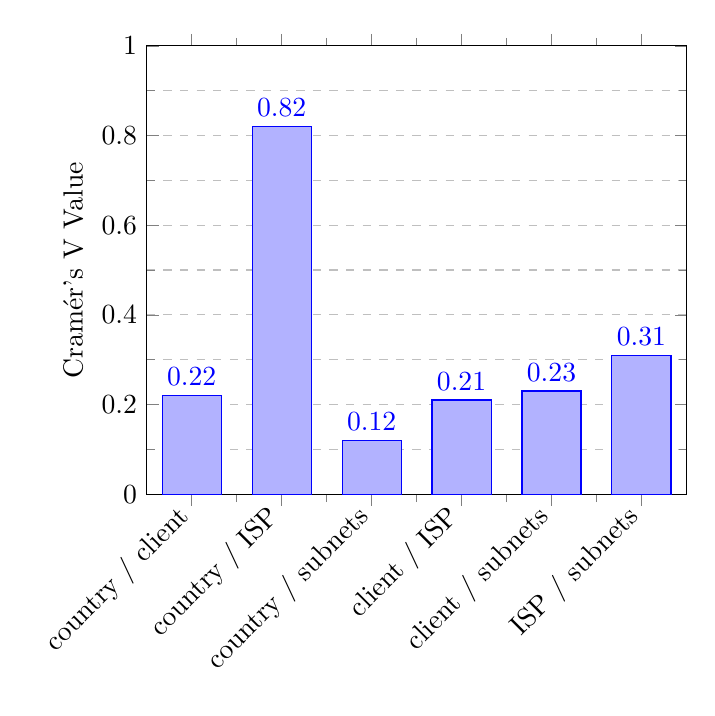
\begin{tikzpicture}
      \begin{axis}[
          ybar,
          bar width=0.75cm, % Adjusted bar width
          ylabel={Cramér's V Value},
          xtick=data,
          xticklabels={
              country / client,
              country / ISP,
              country / subnets,
              client / ISP,
              client / subnets,
              ISP / subnets
          },
          ymajorgrids=true,
          yminorgrids=true,
          grid style=dashed,
          minor x tick num=1,
          minor y tick num=1,
          x tick label style={rotate=45, anchor=east, align=right},
          ymin=0, ymax=1,
          legend pos=north west,
          legend style={font=\footnotesize},
          nodes near coords,
          nodes near coords align={vertical},
          ]
        
          \addplot coordinates {(1, 0.22) (2, 0.82) (3, 0.12) (4, 0.21) (5, 0.23) (6, 0.31)};
        
      \end{axis}
    \end{tikzpicture}
    \caption{Relative level of correlation between attributes}
    \label{fig:relative-level-of-correlation-between-attributes}
\end{figure}

An interesting observation from the results shown in \ref{fig:relative-level-of-correlation-between-attributes} is that there is a relatively low correlation between the country that nodes are based in and the number of attestation subnets that they advertise.  It is widely acknowledged that there is  strong concentration of nodes in the US and EU geographical regions, this low correlation would indicate that nodes that have multiple validators attached to them, and therefore likely to be operated by node operators serving staking pools, may be more geographically distributed.  This hypotheses will require further research however.

\subsection{Correlation between node operator market share and clients and relayers}

The scatter plot in figure \ref{fig:average_client_percentage_by_percentile} show the correlation between the market share of node operators and the average percentage of each client that node operators in the respective market share percentile use.  The 6 main consensus clients are listed in the legend below the chart.  The results displayed in the chart roughly align with the market share of the various clients, and don't reveal any strong correlation to the respective market share of node operators.

The scatter plot in figure \ref{fig:average_relayer_percentage_by_percentile} show the correlation between the market share of node operators and the average percentage of each relayer that node operators in the respective market share percentile use. Again, the results broadly align with the market share of various relayers, and don't reveal any strong correlation.

\begin{figure}[htbp]
  \centering
  \begin{tikzpicture}
    \begin{axis}[
      only marks,
      xlabel={Percentile of Network Penetration},
      ylabel={Percentage Client Use},
      symbolic x coords={0, 1, 2, 3},
      xtick=data,
      xmajorgrids=true,
      ymajorgrids=true,
      grid style=dashed,
      xminorgrids=true,
      yminorgrids=true,
      minor x tick num=1,
      minor y tick num=1,
      legend style={at={(0.5,-0.225)},anchor=north,font=\footnotesize,draw=gray!50,
                    legend columns=3,
                    /tikz/every even column/.append style={column sep=0.5cm},
                    /tikz/every odd column/.append style={column sep=0.5cm}},
      legend entries={Nimbus,Prysm,Lighthouse,Teku,Lodestar,Unknown},
    ]

    \pgfplotstableread[col sep=comma]{data/average_client_percentage_by_percentile.csv}\datatable

    \foreach \col in {1,...,6} {
      \pgfplotstablegetcolumnnamebyindex{\col}\of\datatable\to\colname
      \addplot table[x=Network Penetration, y index=\col] {\datatable};
    }

    \end{axis}
  \end{tikzpicture}
  \caption{Average Client Percentage by Node Operator Market Share}
  \label{fig:average_client_percentage_by_percentile}
\end{figure}

An interesting exercise for future work is to apply the same analysis to staking pools instead of node operators, measuring any correlation between their market share and the clients and relayers they use.
Another interesting measurement would involve looking at data from dataset B, including geographical region, and public cloud provider.  This analysis is not currently possible with the data currently available.

\begin{figure}[htbp]
  \centering
  \begin{tikzpicture}
    \begin{axis}[
      only marks,
      xlabel={Percentile of Network Penetration},
      ylabel={Percentage Client Use},
      symbolic x coords={0, 1, 2, 3},
      xtick=data,
      xmajorgrids=true,
      ymajorgrids=true,
      grid style=dashed,
      xminorgrids=true,
      yminorgrids=true,
      minor x tick num=1,
      minor y tick num=1,
      legend style={at={(0.5,-0.225)},anchor=north,font=\footnotesize,draw=gray!50,
                    legend columns=3,
                    /tikz/every even column/.append style={column sep=0.5cm},
                    /tikz/every odd column/.append style={column sep=0.5cm}},
      legend entries={Manifold,No mev-boost,Agnostic,Aestus,Bloxroute Regulated,Eden Network,Ultra Sound Money,Bloxroute Maxprofit,Flashbots},
    ]

    \pgfplotstableread[col sep=comma]{data/average_relayer_percentage_by_percentile.csv}\datatable

    \foreach \col in {1,...,9} {
      \pgfplotstablegetcolumnnamebyindex{\col}\of\datatable\to\colname
      \addplot table[x=Network Penetration, y index=\col] {\datatable};
    }

    \end{axis}
  \end{tikzpicture}
  \caption{Average Relayer Percentage by Percentile}
  \label{fig:average_relayer_percentage_by_percentile}
\end{figure}

\subsection{Ranking the level of correlation between attributes}

Our analysis attempts to rank the level of correlation between the various attributes in dataset B, pertaining to individual nodes on the network.  The results are visualized in figure \ref{fig:attribute-correlation-ranking}, as a scatter-plot chart.  The y-axis represents the count of occurrences of the value for each attribute for each record and the x-axis represents the sum of all counts for each attribute for each record.  This process is explained in detail in section III, subsection F.

\vspace{6pt}

\begin{figure}[htbp]
    \centering
    \LARGE \textcolor{bluebullet}\textbullet\ \normalsize Country % \ % \
    \LARGE \textcolor{redbullet}\textbullet\ \normalsize Client % \ % \
    \LARGE \textcolor{yellowbullet}\textbullet\ \normalsize ISP % \ % \
    \LARGE \textcolor{greenbullet}\textbullet\ \normalsize Subnets
    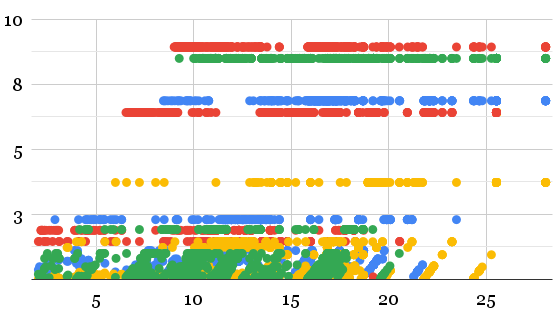
\includegraphics[width=1\linewidth]{figures/node-correlation-ranking.png}
    \caption{Ranking the level of correlation between attributes}
    \label{fig:attribute-correlation-ranking}
\end{figure}

As can be seen from the scatter-plot in figure \ref{fig:attribute-correlation-ranking}, the attributes that show the greatest levels of correlation can be found in the top-right hand of the chart.  These attributes are client, country and subnets.

While we would expect to see a high level of correlation between nodes with reference to clients, largely due to the fact that there are only 6 clients in a population of 1,884 nodes, the fact that there is also a high level of correlation among the country and subnets fields may be significant.

The subnets field relates the number of attestation subnets that each node advertises.  Nodes by default advertise 2 attestation subnets, and this dataset filters out these nodes, leaving only the nodes that advertise 3 or more subnets.  An increase in the level of attestation subnets that a node advertises is presumed to indicate that the node in question is a validator node.

The high level of correlation in both the country field and advertised subnets field may indicate that there is a concentration in terms of geographical location of validator nodes.  This corresponds broadly with the observed geographical centralization in network nodes in general.

\section{Conclusion}

\section{Future Work}

In the future the same model can be applied to Layer 2 rollups as they start to decentralize their sequencers.  When this starts to happen, we may have a scenario where some L2s will have a large market share, but will be fully centralized, where other L2s will have a smaller market share and will have fully decentralized sequencers and/or provers.  In this scenario, simply measuring decentralization via observing the relative market share of each L2 is insufficient to capture the effective level of decentralization within the ecosystem.



% use section* for acknowledgment
\section*{Acknowledgment}


The authors would like to thank...


% Can use something like this to put references on a page
% by themselves when using endfloat and the captionsoff option.
\ifCLASSOPTIONcaptionsoff
  \newpage
\fi

\end{document}
